\documentclass[11pt]{article}
\usepackage{geometry}
\geometry{a4paper}
\usepackage{graphicx}
\usepackage{amsmath}
\usepackage{hyperref}

\title{Cache-Aware Memory Allocator}
\author{Rylie Anderson, Ethan Chapman \\ United States Air Force Academy}
\date{\today}

\begin{document}
\maketitle

\begin{abstract}
This paper presents the design and implementation of a custom cache-aware memory allocator designed to optimize cache hit rate, with hopes of improving performance on modern hardware architectures. We discuss the rationale behind the approach, the specific strategies employed, as well as test results.
\end{abstract}

\section{Introduction}
blah blah blah talk about problems with malloc and how it doesnt care about the cache right now.

\section{Motivation}
maybe just combine this with intro or go deeper into how we can improve

\section{Design}
Talk about the buddy tree!!! Super cool figure:

\begin{figure}[ht]
\centering
\label{fig:tree1}
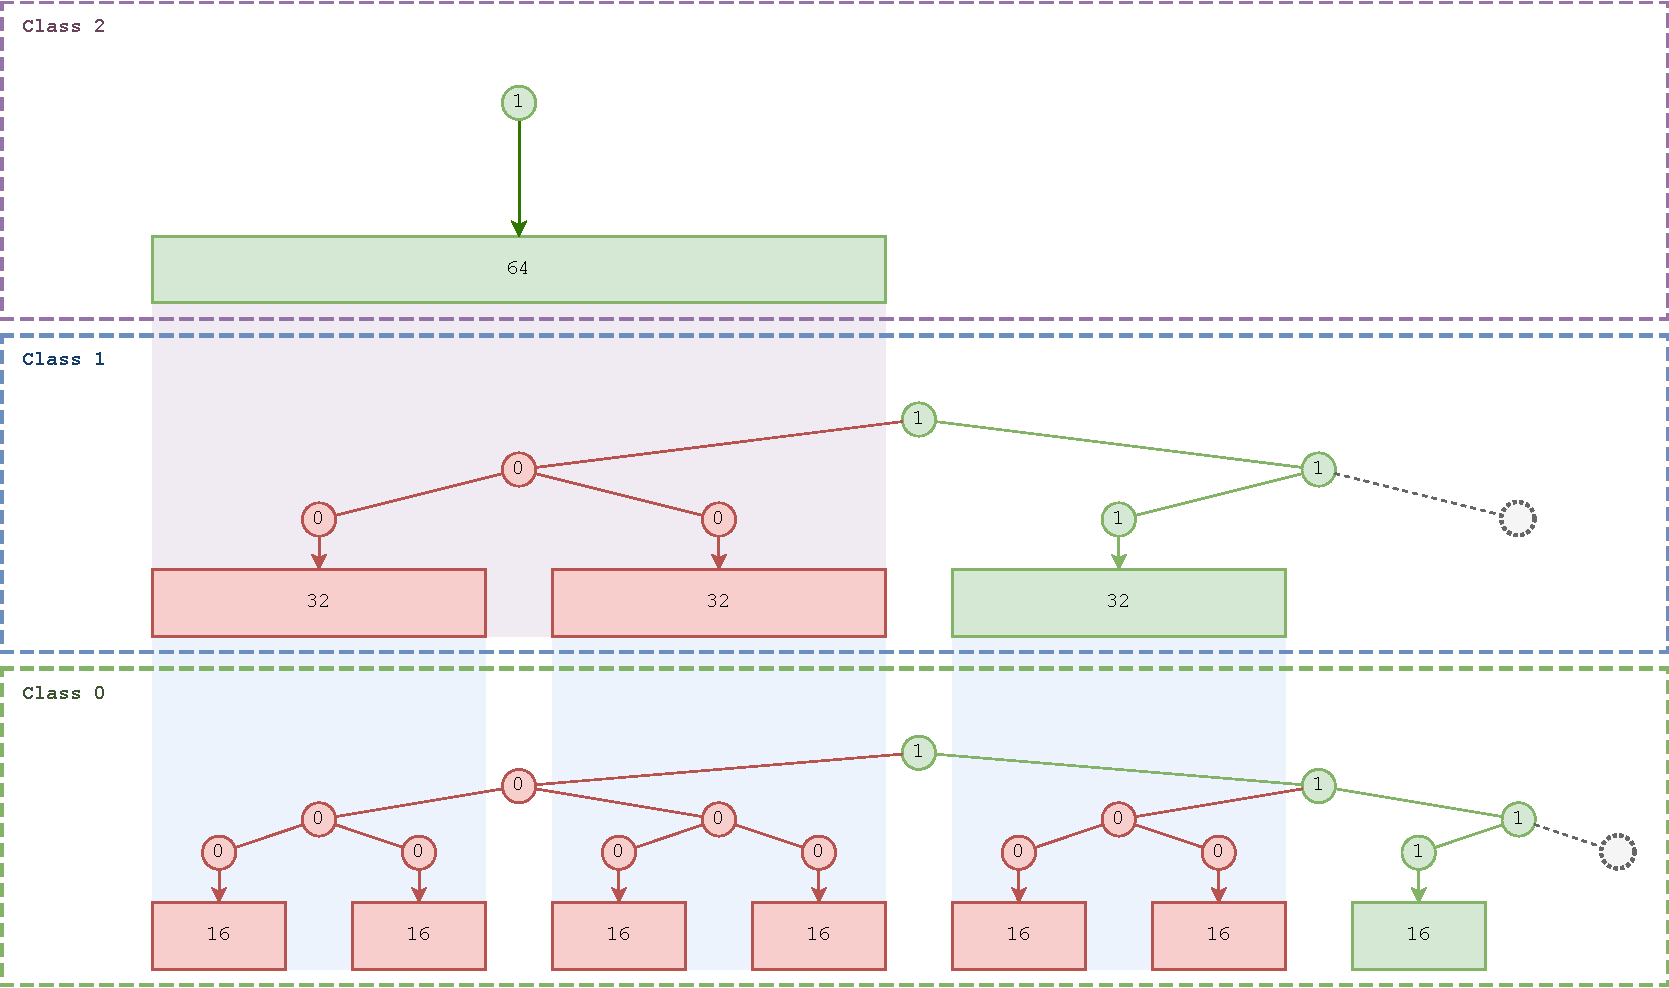
\includegraphics[width=0.5\columnwidth]{tree}
\caption{Starting state of thing}
\end{figure}

Yay that figure is really cool!! We should consider adding more.

\section{Implementation}
Rylie you should talk about the C code details here a bit (but not too much since people dont need all the details)

\section{Testing and Evaluation}
TODO I need to actually test and evaluate.

\section{Conclusion}
In conclusion we actually aren't smarter than malloc people (yet)

\bibliographystyle{plain}
\bibliography{references}

\end{document}
